\section{Auswertung}
\label{sec:Auswertung}

Einem eingetselltes sinusförmiges Signal von $U_{sig} = FEHLT$ mit einer Frequenz von $1 kHz$,
wird mit einem Referenzsignal $U_{ref} = FEHLT$ identischer Frequenz gemischt.
Durch Phasenverschiebung der beiden Signale werden Folgende Ausgangssignale erzeugt.

\begin{figure}
  \centering
  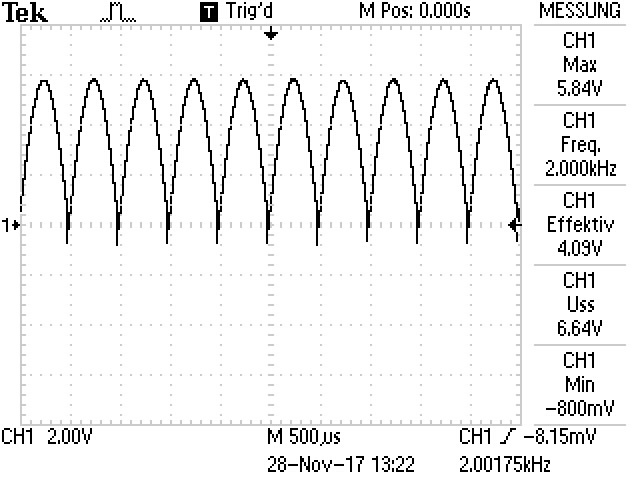
\includegraphics{Phase1.jpg}
  \caption{Phasenverschiebung von 0 Grad.}
  \label{fig:Phase1}
\end{figure}

\begin{figure}
  \centering
  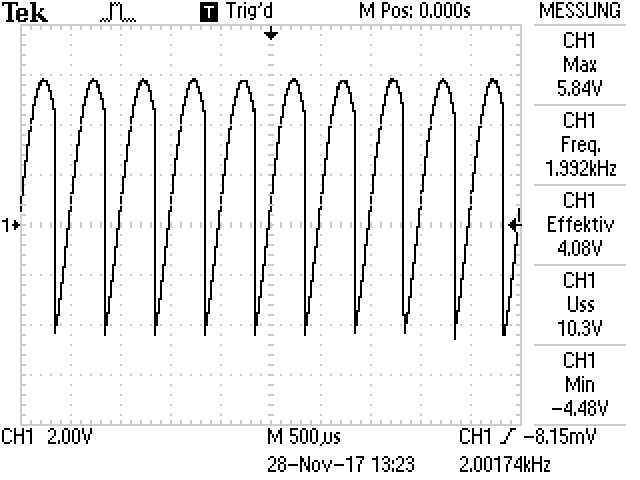
\includegraphics{Phase2.jpg}
  \caption{Phasenverschiebung von FEHLT Grad.}
  \label{fig:Phase2}
\end{figure}

\begin{figure}
  \centering
  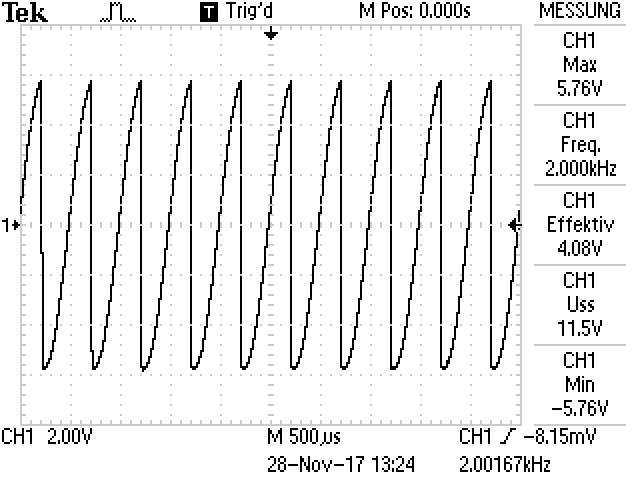
\includegraphics{Phase3.jpg}
  \caption{Phasenverschiebung von FEHLT Grad.}
  \label{fig:Phase3}
\end{figure}

\begin{figure}
  \centering
  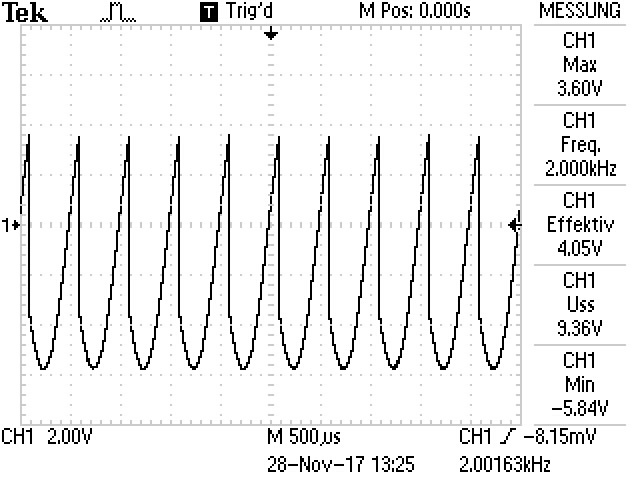
\includegraphics{Phase4.jpg}
  \caption{Phasenverschiebung von FEHLT Grad.}
  \label{fig:Phase4}
\end{figure}

\begin{figure}
  \centering
  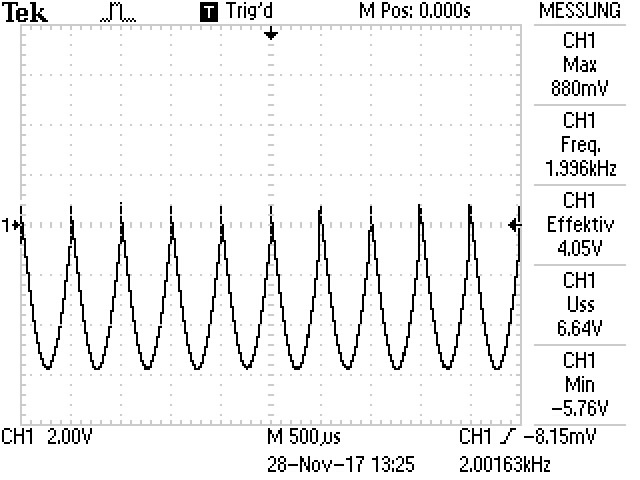
\includegraphics{Phase5.jpg}
  \caption{Phasenverschiebung von 180 Grad.}
  \label{fig:Phase5}
\end{figure}

Es wird eine Umkippung der Amplitude nach 180 Grad festgestellt. 
Mit der Betrachtung der Abbildungen zwischen 0 und 180 Grad wird ein Verlauf der Umkippung erkennbar.
Die Amplitude schlägt weiter nach unten aus, der Verlauf wird spitzer an den oberen Extrema, bis die unteren sich langsam wieder krümmen und schließlich, ein an der Spannungs-Achse gespiegeltes, Bild entsteht. 

\begin{figure}
  \centering
  \includegraphics{plot1.pdf}
  \caption{Verhältnis der Ausgangsspannung zur Phasenverschiebung.}
  \label{fig:plot1}
\end{figure}

\begin{figure}
  \centering
  \includegraphics{plot2.pdf}
  \caption{Verhältnis der Ausgangsspannung zum Abstand der Leuchtdiode, logarithmisch aufgetragen.}
  \label{fig:plot2}
\end{figure}
